The Smart Hosptial Management Tools website is a culmination of multiple websites and software tools used by UT Arlington's Smart Hospital. The product focuses on procedure and work scheduling, allowing users of the tools to track, who, what, and where aspects are scheduled for a hospital procedure, along with inventory management.

\subsection{Features \& Functions}
The homepage of the toolset will allow a user to visit sections of the website that they are allowed access to. A student, for instance, should be able to visit the scheduling area and request procedures that would be approved by a manager or director. A management section, as seen in the early first concept screen shot, permits item tracking and medicine stock views. A calendar will contain scheduled events that keep track people and items that may be used at any specific time. Faculty workers can also use the website to clock in and clock out at manager specified locations based on ip addresses. Finally, a portion of tools will allow managers and teachers to look over reports including worker schedules, hours worked, time for procedures, and procedure participants.

\subsection{External Inputs \& Outputs}
Users shall be able to create accounts including an email and password. Other account details are optional.  Inventory Managers will be able to add or delete items to the inventory database by either uploading a file containing required data for large groups or individually on the list page. Managers can create procedures for students and teachers to participate in. Managers can also export a faculty worker hour sheet at the press of a button.

\subsection{Product Interfaces}
The main input from users will be user account creation, procedure events and inventory additions. Account creation will include fields for Name, Email, Password. Administrators will have the ability to elevate users to managers or admin. The entire website will be an input interface.

\begin{figure}[h!]
	\centering
   	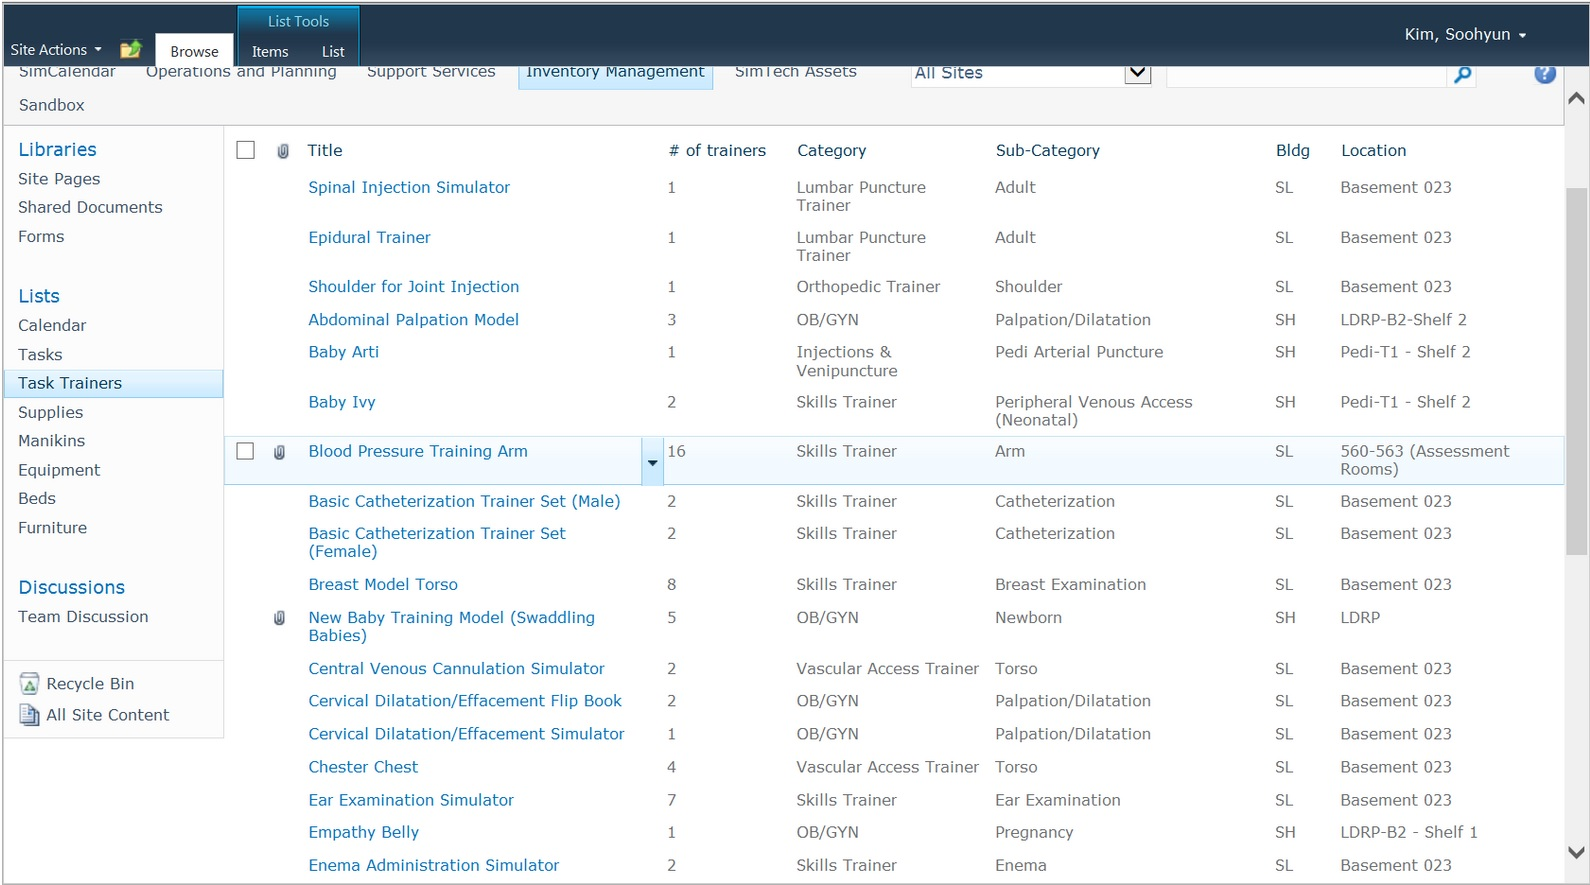
\includegraphics[width=0.75\textwidth]{images/concept_database}
    \caption{The current uta smart hospital database list to be incorporated to the management tools}
\end{figure}